\documentclass[hidelinks,onefignum,onetabnum,final]{siamart220329}  % for arxiv
%\documentclass[review,hidelinks,onefignum,onetabnum,final]{siamart220329}  % for submission

\usepackage{amsfonts,yhmath}
\usepackage{graphicx}
\usepackage{epstopdf}
\ifpdf
  \DeclareGraphicsExtensions{.eps,.pdf,.png,.jpg}
\else
  \DeclareGraphicsExtensions{.eps}
\fi

% Used for creating new theorem and remark environments
\newsiamremark{remark}{Remark}
\newsiamthm{claim}{Claim}
%\newsiamthm{conjecture}{Conjecture}
\newsiamremark{example}{Example}

\newcommand{\newindthm}[2]{
  \theoremstyle{plain}
  \theoremheaderfont{\normalfont\sc}
  \theorembodyfont{\normalfont\itshape}
  \theoremseparator{.}
  \theoremsymbol{}
  \newtheorem{#1}{#2}
}
\newindthm{conjecture}{Conjecture}
\renewcommand{\theconjecture}{\Alph{conjecture}}

\usepackage{amsopn}
\DeclareMathOperator{\diag}{diag}

\usepackage{bm,bbm,empheq,verbatim,fancyvrb,amssymb}
\usepackage{booktabs,multirow,xspace}
\usepackage{pifont}

\usepackage{tikz}
\usetikzlibrary{decorations.pathreplacing}
\usetikzlibrary{graphs,quotes}

\newcommand{\eps}{\epsilon}
\newcommand{\RR}{\mathbb{R}}

\newcommand{\grad}{\nabla}
\newcommand{\Div}{\nabla\cdot}

\newcommand{\bbf}{\mathbf{f}}
\newcommand{\bg}{\mathbf{g}}
\newcommand{\bn}{\mathbf{n}}
\newcommand{\bu}{\mathbf{u}}
\newcommand{\bv}{\mathbf{v}}
\newcommand{\bw}{\mathbf{w}}
\newcommand{\bx}{\mathbf{x}}
\newcommand{\bz}{\mathbf{z}}

\newcommand{\bX}{\mathbf{X}}

\newcommand{\bzero}{\bm{0}}

\newcommand{\btau}{\bm{\tau}}

\newcommand{\cB}{\mathcal{B}}
\newcommand{\cH}{\mathcal{H}}
\newcommand{\cK}{\mathcal{K}}
\newcommand{\cQ}{\mathcal{Q}}
\newcommand{\cV}{\mathcal{V}}
\newcommand{\cX}{\mathcal{X}}

\newcommand{\hcK}{\widehat{\cK}}

\newcommand{\nn}{{\text{\textnormal{n}}}}
\newcommand{\pp}{{\text{\textnormal{p}}}}
\newcommand{\qq}{{\text{\textnormal{q}}}}
\newcommand{\rr}{{\text{\textnormal{r}}}}

\newcommand{\ip}[2]{\left<#1,#2\right>}

\newcommand{\XX}{\ding{55}}

\newcommand{\dx}{\, \mathrm{d}x}

\newcommand{\rhoi}{\rho_{\text{i}}}

\DeclareMathOperator*{\argmin}{arg\,min}
\DeclareMathOperator*{\Hull}{Hull}

\newcommand{\Vdiv}{\cV_{\text{\textnormal{div}}}}


% running headers and PDF metadata
\headers{Bounds on geometry errors in glacier simulations}{E. Bueler}

\title{Bounds on geometry errors in glacier simulations}

\author{Ed Bueler\thanks{Department of Mathematics and Statistics, University of Alaska Fairbanks, USA (\email{elbueler@alaska.edu}).}}


\begin{document}
\maketitle

\begin{abstract}
The primary data which determine the evolution of glaciation are bedrock elevation and surface mass balance.  From this data the glacier's geometry solves a free-boundary problem over a set of admissible surface elevation functions.  Admissibility requires that the ice surface is above the bedrock topography, equivalently that the ice thickness is nonnegative.  For an implicit time step, the free-boundary problem can be posed in weak form as a variational inequality over a fixed map-plane region.  We conjecture that these continuous-space problems are well-posed in the case of non-shallow Stokes dynamics.  We show an abstract estimate for finite element approximations of variational inequality problems over Banach spaces, a theorem in which the nonlinear operator is assumed to be coercive and Lipshitz.  When applied in the glacier case, all terms in the error estimate can be physically-interpreted, and practical approaches to bound and/or reduce these errors are proposed.  The resulting computable bounds on the geometry approximation error are demonstrated in an implicit time-stepping glacier simulation based on Stokes dynamics.
\end{abstract}

% REQUIRED
\begin{keywords}
error bounds, finite element methods, glaciers, ice flow, variational inequalities
\end{keywords}

% REQUIRED
%\begin{MSCcodes}
%FIXME
%\end{MSCcodes}


\section{Introduction} \label{sec:intro}

Glacier and ice sheet simulations typically model the ice as a layer of free-surface, very-viscous, incompressible, and non-Newtonian fluid \cite{GreveBlatter2009,SchoofHewitt2013}.  For simplicity we will restrict our considerations to simulations of glaciers on land, without floating portions.  Note that an ``ice sheet'' is simply a continent-scale glacier.

The two types of essential input data into such simulations are the bedrock elevation, which is assumed to be constant in time, and the time-dependent surface mass balance (SMB; $=$ climatic mass balance \cite{Cogleyetal2011}) rate.  By definition, the SMB is the annually-averaged difference of vertically-accumulating snow minus the loss of (liquid) water, through runoff, at the upper surface of the glacier \cite{Cogleyetal2011}.  Note that elevations are measured here in meters, and SMB is measured in ice-equivalent units of meters per second.

Thus a glacier simulation at least takes the bedrock topography, a time-dependent climate, and an initial glacier geometry as inputs.  It produces the glacier's evolving geometry and flow velocity; these output fields are of primary scientific value.  The geometry is parameterized by either the (upper) surface elevation or the ice thickness.  The computed flow velocity is, however, only defined at those locations and times where ice is present, on the evolving 3D domain between the bedrock and surface elevations.

Additional complications are common in comprehensive ice sheet models \cite{SchoofHewitt2013}.  For example, the internal energy of the ice \cite{Aschwandenetal2012}, and/or liquid water within the ice matrix, or at ice surfaces, may be tracked.  However, we only consider conservation of mass and momentum, but not energy conservation nor liquid/solid (two phase) models.  On the other hand, we will not make the shallowness assumptions which are common in comprehensive models.

At a time and map-plane location where a glacier exists the surface elevation exceeds the bedrock elevation, equivalently the ice thickness is positive.  That is, the glacier's geometry must satisfy an inequality to be admissible.  To introduce our inequality-constrained problem for geometry we start with the notation sketched in Figure \ref{fig:stokesdomain}.

\medskip
\begin{figure}[ht]
\centering
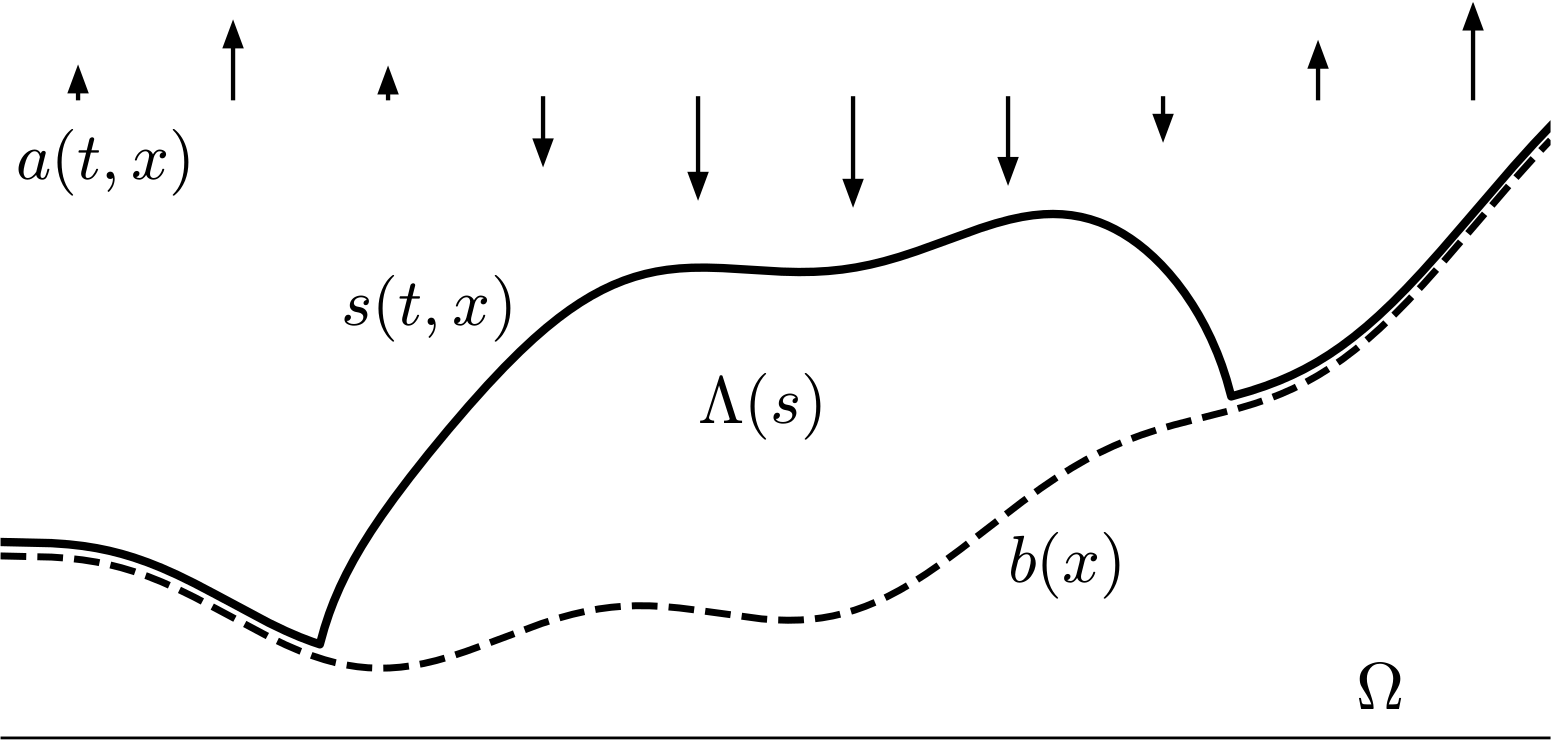
\includegraphics[width=0.65\textwidth]{genfigs/stokesdomain.pdf}
\caption{Glacier notation used in this paper.}
\label{fig:stokesdomain}
\end{figure}

\medskip
Let $\Omega \subset \RR^2$ be a fixed portion of land.  Let $x=(x_1,x_2)\in\Omega$ denote the map-plane coordinate(s).  Assume that we are given, as data, a bed elevation function $b(x)$ for $x\in\Omega$ and an SMB function $a(t,x)$ for $t\in [0,T]$ and $x\in \Omega$.

Note that $a$ is generally signed, and in areas where $a>0$ (accumulation; downward arrows in Figure \ref{fig:stokesdomain}) then a glacier will exist.  If $a<0$ (upward arrows) then either a glacier exists with an ablating surface, or no glacier exists.  Determining which situation applies at a given point $t,x$ requires solving the free-boundary problems considered in this paper.

Let $s(t,x)$ be the (solution) ice surface elevation.  We will regard this as defined everywhere, subject to the constraint that the surface $z=s(t,x)$ must be at or above the bedrock: $s(t,x) \ge b(x)$.  In regions with no ice we set $s(t,x)=b(x)$.  The solution ice velocity $\bu(t,x,z)$ and pressure $p(t,x,z)$ are then defined only on the 3D domain
\begin{equation}
\Lambda(t) = \left\{(x,z)\,:\,b(x) < z < s(t,x)\right\} \subset \Omega \times \RR. \label{eq:icydomain}
\end{equation}
This aspect of glacier modeling deserves emphasis: at any time $t$ the 3D domain $\Lambda(t)$, on which the velocity and pressure can be meaningful, is determined by the time-dependent surface elevation $s(t,x)$, which is itself part of the model solution.

The surface trace of the ice velocity will be of importance, and we define it using extension by zero, so that it is defined everywhere in $\Omega$.  Let
\begin{equation}
\bu|_s(t,x) = \begin{cases} \bu(t,s,s(t,x)), & s(t,x)>b(t,x) \\
                            0, & \text{otherwise} .\end{cases} \label{eq:defineus}
\end{equation}
(That is, $\bu|_s=0$ by definition in ice-free areas.)  Also let $\bn_s = \left<-\grad s,1\right>$, which is an (un-normalized) upward surface normal vector.

For any $T>0$, an infinite-dimensional nonlinear complementarity problem (NCP) \cite{Bueler2021conservation,FacchineiPang2003,SchoofHewitt2013} applies almost everywhere in $[0,T]\times \Omega$:
\begin{subequations}
\label{eq:ncp}
\begin{align}
s - b &\ge 0 \\
\frac{\partial s}{\partial t} - \bu|_s \cdot \bn_s - a &\ge 0 \\
(s - b) \left(\frac{\partial s}{\partial t} - \bu|_s \cdot \bn_s - a\right) &= 0
\end{align}
\end{subequations}
This strong form NCP statement will be reformulated as a variational inequality (VI; \cite{KinderlehrerStampacchia1980}) in Section \ref{sec:model} below.  It says that either a location is ice free ($s-b=0$), where the climate is locally ablating ($a\le 0$), or that the surface kinematical equation (SKE) holds:
\begin{equation}
\frac{\partial s}{\partial t} - \bu|_s \cdot \bn_s - a = 0.  \label{eq:ske}
\end{equation}
SKE \eqref{eq:ske} says that the (non-material) surface of the ice moves vertically according to the sum of a component of the ice velocity at the surface and the SMB \cite{SchoofHewitt2013}.  Equation \eqref{eq:ske} is a statement of mass conservation at a non-material surface \cite{Aschwandenetal2012}, sometimes wrongly\footnote{Equation \eqref{eq:ske} is not the boundary condition for any identifiable problem.} called a ``kinematical boundary condition'' \cite{GreveBlatter2009}.

In the current paper the SMB $a(t,x)$ is necessarily assumed to be defined everywhere in $\Omega$, regardless of whether a glacier is present or not.  At an ice-free location the value $a(t,x)$ can be modeled using precipitation and an energy balance \cite{GreveBlatter2009}, for instance by hypothesizing an ice or snow surface and then computing the balance of snow accumulation minus the total ablation from the available energy for melt.  Because a simulated glacier can advance into unglaciated locations, the provided SMB there should have the value which a glacier surface would experience at that time and (3D) location.

The continuum models considered in this paper conserve mass and momentum.   The (standard) non-shallow ice dynamics model used here is a non-sliding (e.g.~frozen) base, isothermal, shear-thinning (non-Newtonian), and incompressible Stokes problem \cite{GreveBlatter2009,JouvetRappaz2011,SchoofHewitt2013}.  Regarding the domain for this model, recall definition \eqref{eq:icydomain} and let $\Gamma_s(t) \subset \partial \Lambda(t)$ be the upper surface $z=s$ and $\Gamma_b(t) \subset \partial \Lambda(t)$ be the base $z=b$.  The possibility of cliffs at the ice margin is neglected, so $\partial \Lambda(t) = \overline{\Gamma_s(t)} \cup \overline{\Gamma_b(t)}$ at any time.

To state the shear-thinning Glen's flow law, let $D\bu=(\grad \bu + \grad \bu^{\top})/2$ denote the strain rate tensor, with Frobenius norm $|D\bu| = (D\bu:D\bu)^{1/2} = \left((D\bu)_{ij} (D\bu)_{ij}\right)^{1/2}$.  The effective ice (dynamic) viscosity \cite{GreveBlatter2009} is given by a regularized formula
\begin{equation}
\nu(D\bu) = \nu_\pp \left(|D\bu|^2 + \eps\right)^{(\pp-2)/2} \label{eq:glen}
\end{equation}
The exponent $1 < \pp \le 2$, often written $\pp=(1/\nn)+1$, is approximately 4/3.  The coefficient $\nu_\pp>0$ has $\pp$-dependent units, but $\nu(D\bu)$ has SI units $\text{kg}\,\text{m}^{-1}\,\text{s}^{-1}$.  The value of $\nu_\pp$ can be determined from measured properties of ice \cite{GoldsbyKohlstedt2001,GreveBlatter2009}, including temperature, but it is assumed to be constant (isothermal) here.  Note that $\pp=2$ yields a Newtonian fluid with constant viscosity, while for $\pp < 2$ the $\eps>0$ regularization implies that $\nu(D\bu)$ is bounded above.

Assume that the density of ice $\rhoi$ and the acceleration of gravity $\bg$ are constant.  At each time $t$ the modeled glacier has velocity and pressure solving the following 3D fluid equations:
\begin{subequations}
\label{eq:stokes}
\begin{align}
- \nabla \cdot \left(2 \nu(D\bu)\, D\bu\right) + \nabla p &= \rhoi \bg && \text{within $\Lambda(t)$} \\
\nabla \cdot \bu &= 0 && \qquad \text{''} \label{eq:stokes:incomp} \\
\left(2 \nu(D\bu) D\bu - pI\right) \bn_s &= \bzero && \text{on $\Gamma_s(t)$}\label{eq:stokes:stressfreesurface} \\
\bu  &= \bzero && \text{on $\Gamma_b(t)$}
\end{align}
\end{subequations}
Note that boundary condition \eqref{eq:stokes:stressfreesurface} says that the sub-aerial upper surface is stress free; this should not be confused with \eqref{eq:ske}.

In summary at this point, a glacier simulation is an evolving free-surface flow, subject to a signed climate that can add or remove ice, coupled to a nonlinear Stokes problem which must be solved within an evolving, 3D icy domain.  A well-posed initial/boundary value problem for \eqref{eq:icydomain}--\eqref{eq:stokes} will require data $b(x),a(t,x)$ plus an initial surface elevation $s(0,x)$.  The solution variables are $s(t,x)$, $\bu(t,x,z)$, and $p(t,x,z)$, with $s$ defined everywhere over $[0,T]\times \Omega$, but subject to $s \ge b$, and with $\bu,p$ defined on $\Lambda(t)$ for each $t$.  The surface elevation $s$ and surface velocity $\bu|_s$ are linked by the kinematical NCP \eqref{eq:ncp}, in which the time derivative appears.  The Stokes sub-model \eqref{eq:glen}--\eqref{eq:stokes} acts as an instantaneous\footnote{It acts instantaneously because the flow is very viscous \cite{Acheson1990}.} ``algebraic'' constraint on the evolution statement in \eqref{eq:ncp}.  The coupled, infinite-dimensional problem \eqref{eq:icydomain}--\eqref{eq:stokes} is therefore both a differential algebraic equation (DAE) system \cite{AscherPetzold1998} and an NCP.

One must choose whether the glacier geometry is parameterized by surface elevation or thickness.  While essentially equivalent in the (continuum) problem, formulations using these different functions have different character when the bedrock is realistically rough.  Specifically, when applying the abstract estimate of Section \ref{sec:abstractestimate}, surface elevation $s$ is preferred because of the flow-caused smoothing effect illustrated in Figure \ref{fig:giscross}.  We observe that for land-based glaciers $s(t,x)$ is smoother in $x$ than the thickness $H(t,x) = s(t,x)-b(x)$ because the latter ``inherits'' the lower regularity of the (typically) eroded and/or faulted bedrock topography $b(x)$.

\begin{figure}
\begin{minipage}[t]{0.85\textwidth}
\vspace{0pt}
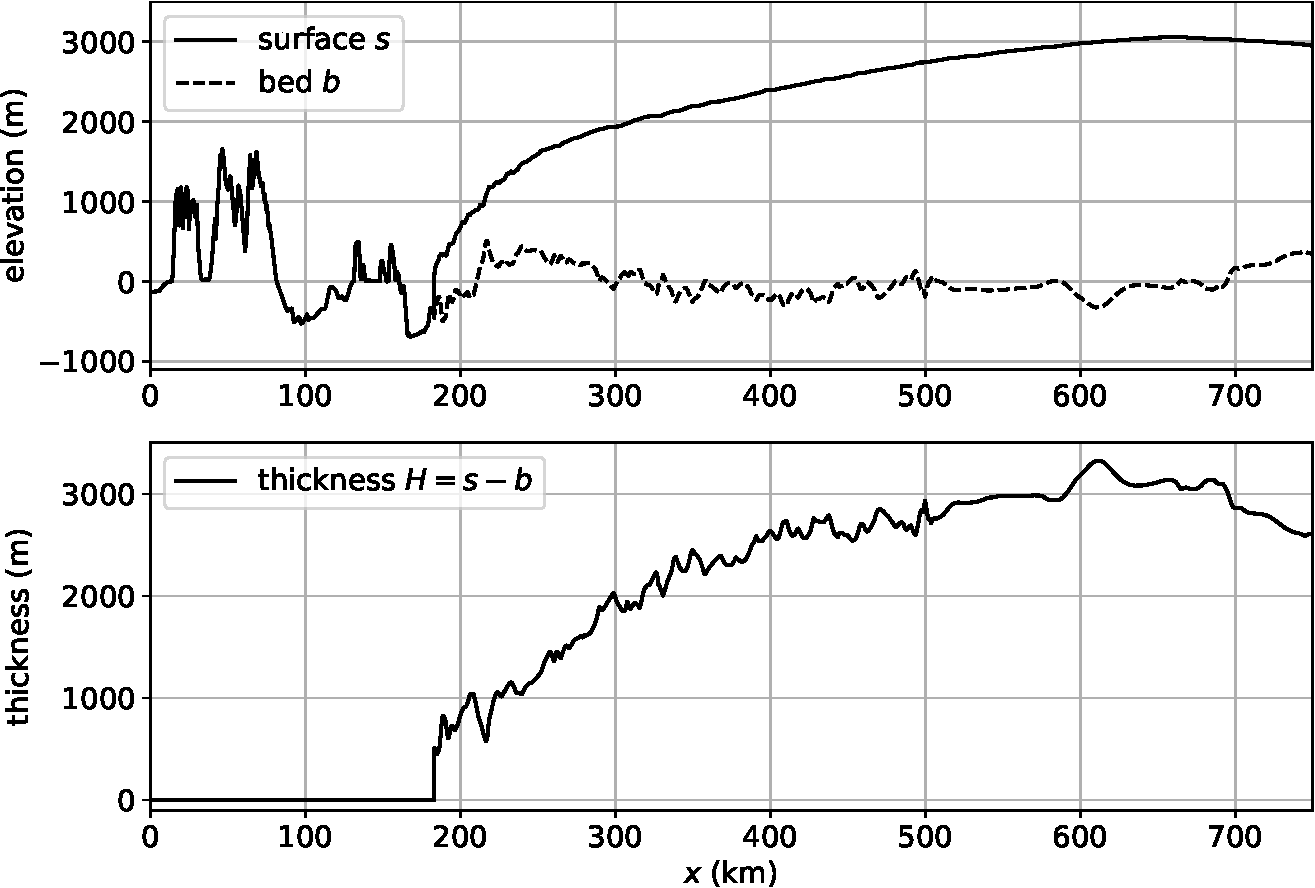
\includegraphics[width=\textwidth]{genfigs/giscross.pdf}
\end{minipage}
\,
\begin{minipage}[t]{0.13\textwidth}
\vspace{10pt}
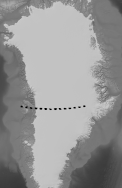
\includegraphics[width=\textwidth]{genfigs/gis/gris-profile-gray.png}
\end{minipage}
\caption{A cross-section of the Greenland ice sheet at $70^\circ$N latitude (inset).  While the ice surface $s$ is relatively smooth because of ice flow (top), the bedrock elevation $b$ is much rougher.  The corresponding ice thickness $H = s-b$ (bottom), though a valid geometry parameterization, inherits the low regularity of $b$.  (Data from \cite{Morlighemetal2017} and A.~Aschwanden, personal communication.)}
\label{fig:giscross}
\end{figure}

Glacier simulations are commonly formulated using a finite element (FE) method for the Stokes sub-problem \cite{IsaacStadlerGhattas2015,Jouvetetal2008,Pattynetal2008}, or for a shallow approximation thereof.  However, to the author's knowledge all existing non-shallow (Stokes) evolution models use a explicit time-stepping scheme for the geometry, for example as in \cite{Jouvetetal2008} or \cite{LofgrenAhlkronaHelanow2022}, with the one exception of the exploratory model in reference \cite{WirbelJarosch2020}.  In the current paper we consider implicit time steps, for theoretical reasons addressed here, and for simulation performance reasons laid out in \cite{Bueler2023}.

FIXME: WHAT WE ACCOMPLISH

This paper is organized as follows.  Section \ref{sec:stokes} recalls the existing theory of Glen-law Stokes problems on fixed domains, but we add an apparently-new bound on the surface trace of the velocity solution (Corollary \ref{cor:surfacetracebound}).  In Section \ref{sec:model} we reformulate the coupled problem \eqref{eq:icydomain}--\eqref{eq:stokes} as a VI weak form for an implicit (backward Euler) time step.  The key coupling term in this problem is the surface motion term $\bu|_s\cdot \bn_s$ in the SKE, for which we provide a quantitative bound (Lemma \ref{lem:philipschitz}), over a Sobolev space of surface elevation functions, subject to a conjecture that the surface trace of velocity is Lipschitz continuous with respect to surface elevation.  Well-posedness for each implicit time-step problem is considered in Section \ref{sec:theory}, including a second conjecture on the coercivity of the surface motion term.  Certain physical and modeling ideas are discussed here, as context needed to understand these conjectures.  At this point we have in hand a mathematically-precise, time-discretized continuum model, though one with only conjectural well-posedness; see Theorem \ref{thm:stepwellposed}.  This continuum model, precisely stated for what we believe is the first time, is one which can be approximated by a finite element (FE) method, thereby simulating the (non-shallow) evolution of glacier geometry via implicit time steps.  In Section \ref{sec:abstractestimate} we prove an abstract FE error estimate, namely Theorem \ref{thm:abstractestimate}, and its corollaries, for general VI problems involving fully-nonlinear operators on Banach spaces.  This new estimate, which makes coercive and Lipshitz assumptions, extends the classical case by Falk \cite{Falk1974} for bilinear forms.  In Section \ref{sec:application} we apply the estimate to the glacier model.  The distinctive character of non-sliding land-based glaciers, in terms of how they respond to climate (mass balance) perturbations, and how they stagnate as ice thickness approaches zero, implies that certain terms in the error estimate are small.  Computable geometry error upper bounds follow.  These estimates are demonstrated in Section \ref{sec:demo} on an idealized, but non-trivial, glacier simulation implemented in Firedrake \cite{Hametal2023}.


\section{On the surface velocity from a Stokes problem} \label{sec:stokes}

In this Section we consider the weak form of the non-sliding, isothermal, and Glen-law Stokes sub-model \eqref{eq:glen}--\eqref{eq:stokes}.  This sub-model is applied on a fixed 3D domain $\Lambda = \Lambda(t)$, defined by \eqref{eq:icydomain}, at a fixed time $t$.  It computes the surface velocity field $\bu|_s$ which appears in NCP \eqref{eq:ncp}, the weak form of which is presented in Section \ref{sec:model} below.

Suitable function spaces for this Stokes problem are well-known so long as the domain $\Lambda$ is sufficiently regular.  We assume that the ice base $\Gamma_b\subset\partial \Lambda$, on which a Dirichlet condition $\bu=\bzero$ holds, has positive measure.  The remaining Neumann boundary $\Gamma_s = \partial \Lambda \setminus \overline{\Gamma_b}$ must be sufficiently-smooth so that a zero normal stress condition can be applied.

Let $1 < \pp \le 2$.  (Recall that $\pp=(1/\nn)+1\approx 4/3$ in viscosity formula \eqref{eq:glen}.)  The Sobolev space \cite{Evans2010} of real-valued functions with $\pp$th-power integrable first derivatives is denoted $W^{1,\pp}(\Lambda)$.  Let
\begin{equation}
\cV = W_b^{1,\pp}(\Lambda; \RR^3) \label{eq:defineV}
\end{equation}
denote the corresponding space of vector-valued functions with value (trace) zero along $\Gamma_b$.  Let $[L]>0$ be a representative \emph{horizontal} glacier dimension.  We define the norm on $\cV$ by
\begin{equation}
\|\bv\|_{\cV} = \left(\int_\Lambda |\bv|^\pp\,dx\,dz + [L]^\pp \int_\Lambda |\grad\bv|^\pp\,dx\,dz\right)^{1/\pp}. \label{eq:vnorm}
\end{equation}
Here $dx\,dz = dx_1\,dx_2\,dz$ is the 3D volume element, which will be suppressed in later integrals over $\Lambda$.  Note that $|\bv|$ denotes the Euclidean norm of $\bv\in\RR^3$ and $|\grad\bv|=\left((\grad\bv)_{ij} (\grad\bv)_{ij}\right)^{1/2}$ is the Frobenius norm of $\grad\bv\in\RR^{3\times 3}$.  Remark 1.2.1 in \cite{BoffiBrezziFortin2013} explains the length scaling in \eqref{eq:vnorm}, so that $\|\bv\|_{\cV}$ has consistent units.

Let $\cQ=L^{\pp'}(\Lambda)$ where $\pp'=\pp/(\pp-1)\approx 4$ is the conjugate exponent.  Define
\begin{equation}
\mathcal{M} = \cV \times \cQ \label{eq:glenstokes:mixedspace}
\end{equation}
as the space of admissible velocity and pressure pairs.  For $(\bu,p) \in \mathcal{M}$ define
\begin{equation}
F_\Lambda(\bu,p)[\bv,q] = \int_\Lambda 2 \nu(|D\bu|) D\bu : D\bv - p \Div\bv - (\Div\bu) q - \rhoi \bg \cdot \bv. \label{eq:glenstokes:fcnl}
\end{equation}
The (mixed) weak form seeks the solution $(\bu,p)$ satisfying
\begin{equation}
F_\Lambda(\bu,p)[\bv,q] = 0 \qquad \text{for all } (\bv,q) \in \mathcal{M}. \label{eq:glenstokes:weak}
\end{equation}

Jouvet and Rappaz \cite{JouvetRappaz2011} have proven that problem \eqref{eq:glenstokes:weak} is well-posed if the Neumann portion of $\partial\Lambda$ is $C^1$.  Their proof uses the equivalence of \eqref{eq:glenstokes:weak} and the minimization of a convex and coercive functional over the divergence-free subspace $\Vdiv = \{\bv\in\cV\,:\,\Div\bv=0\}$.  Our regularization in Glen law \eqref{eq:glen} differs from that in \cite{JouvetRappaz2011}, but the necessary modifications are addressed in \cite{IsaacStadlerGhattas2015}.  Note that if the weak solution is sufficiently regular then the strong form \eqref{eq:stokes} is satisfied.

\begin{theorem} \label{thm:stokeswellposed} \cite[Theorem 3.10]{JouvetRappaz2011} and \cite[Appendix A]{IsaacStadlerGhattas2015}.  Suppose $\Lambda$ is bounded, $\partial\Lambda$ is Lipschitz, $\Gamma_s$ is $C^1$, and $\Gamma_b$ has positive measure.  Let $1<\pp\le 2$ and $\eps>0$ in \eqref{eq:glen}.  Then there exists a unique pair $(\bu,p) \in \mathcal{M}$ solving \eqref{eq:glenstokes:weak}, and $\bu\in \Vdiv$.
\end{theorem}

Our primary purpose, resumed in the next Section, is to study the glacier geometry NCP \eqref{eq:ncp}, and its weak form.  For that analysis we need to bound the surface trace $\bu|_s$ in terms of geometric properties of $\Lambda$.  This uses several inequalities.

\begin{lemma}[Poincar\'e's inequality] \label{lem:poincare}
Under the domain assumptions of Theorem \ref{thm:stokeswellposed}, there exists a dimensionless constant $c_{\pp}(\Lambda)>0$ so that for all $\bv \in \cV$,
\begin{equation}
\int_\Lambda |\bv|^\pp \le c_{\pp}(\Lambda) [L]^\pp \int_\Lambda |\grad\bv|^\pp. \label{eq:poincare}
\end{equation}
\end{lemma}

\begin{lemma}[Korn's inequality] \label{lem:korns}
Under the same assumptions, there exists a dimensionless constant $k_{\pp}(\Lambda)>0$ so that for all $\bv \in \cV$,
\begin{equation}
\int_\Lambda |\grad\bv|^\pp \le k_{\pp}(\Lambda) \int_\Lambda |D\bv|^\pp. \label{eq:korns}
\end{equation}
\end{lemma}

From Lemma \ref{lem:poincare} it follows that $\|\bu\|_{\cV}^\pp \le (c_{\pp}(\Lambda) + 1) [L]^\pp \int_\Lambda |\grad\bv|^\pp$; this is used below.  To prove Lemma \ref{lem:korns}, set $F(x)$ to the identity in Corollary 4.1 of \cite{Pompe2003}.  A similar $\pp$-norm Korn's inequality was earlier proven by Ting \cite{Ting1972}---see Theorem 5.12 in \cite{KikuchiOden1988}---but only for zero Dirichlet conditions over all of $\partial \Lambda$.

The main idea of the following bound is that velocity is controlled by geometric properties of the domain $\Lambda$, including constants in the above inequalities, and physical constants.  It is an exercise for the reader to check unit consistency in this result.

\begin{lemma}[3D \emph{a priori} bound] \label{lem:stokesapriori}
Suppose $\bu\in\cV$ is the Stokes velocity solution from Theorem \ref{thm:stokeswellposed}.  Let $|\Lambda|$ denote the ice volume.  Then:
\begin{equation}
\|\bu\|_{\cV}^\pp \le \left(\frac{\rhoi |\bg| (c_{\pp}(\Lambda) + 1) k_{\pp}(\Lambda)}{2 \nu_\pp}\right)^{\pp'} [L]^{\pp\pp'} |\Lambda|. \label{eq:stokesapriori}
\end{equation}

\end{lemma}

\begin{proof}
From \eqref{eq:glenstokes:weak} and $\bu \in\Vdiv$ it follows that
\begin{equation}
0= F_\Lambda(\bu,p)[\bu,p] = \int_\Lambda 2 \nu(|D\bu|) D\bu : D\bu - \rhoi \bg \cdot \bu.  \label{eq:stokes:substituteu}
\end{equation}
Apply Lemma \ref{lem:korns}, equation \eqref{eq:glen}, equation \eqref{eq:stokes:substituteu}, and H\"older's inequality:
\begin{align}
\int_\Lambda |\grad\bu|^\pp &\le k_{\pp}(\Lambda) \int_\Lambda |D\bu|^{\pp-2} D\bu:D\bu \label{eq:stokes:workapriori} \\
	&\le \frac{k_{\pp}(\Lambda)}{2 \nu_\pp} \int_\Lambda 2 \nu_\pp \left(|D\bu|^2 + \eps\right)^{(\pp-2)/2} D\bu:D\bu \notag \\
	&= \frac{k_{\pp}(\Lambda)}{2 \nu_\pp} \int_\Lambda \rhoi \bg \cdot \bu \notag \\
	&\le \frac{k_{\pp}(\Lambda)}{2 \nu_\pp} \|\rhoi \bg\|_{L^{\pp'}} \|\bu\|_{L^\pp} \notag \\
	&\le \frac{\rhoi |\bg| k_{\pp}(\Lambda)}{2 \nu_\pp} |\Lambda|^{1/\pp'} \|\bu\|_{L^\pp}. \notag
\end{align}
(This assumes that ice density and gravity are constant.)  By the comment after Lemma \ref{lem:poincare}, and the simple fact $\|\bu\|_{L^\pp} \le \|\bu\|_{\cV}$, we have
\begin{align*}
\|\bu\|_{\cV}^\pp \le (c_{\pp}(\Lambda) + 1) [L]^\pp \frac{\rhoi |\bg| k_{\pp}(\Lambda)}{2 \nu_\pp} |\Lambda|^{1/\pp'} \|\bu\|_{\cV}.
\end{align*}
Divide by the norm and raise both sides to the $\pp' = \pp/(\pp-1)$ power to yield \eqref{eq:stokesapriori}.
\end{proof}

\begin{lemma}[Trace inequality] \label{lem:trace}
Under the domain assumptions of Theorem \ref{thm:stokeswellposed}, there exists a dimensionless constant $\gamma_{\pp}(\Lambda)>0$ so that for all $\bv \in \cV$,
\begin{equation}
\int_{\Gamma_s} |\bv|^\pp \,dS \le \frac{\gamma_{\pp}(\Lambda)}{[L]} \|\bv\|_{\cV}^\pp \label{eq:trace}
\end{equation}
where $\bv$ on the left is the trace on $\Gamma_s$.
\end{lemma}

\begin{proof}
Theorem 5.5.1 in \cite{Evans2010} defines a trace operator $T:\cV\to L^\pp(\partial\Lambda)$, and a constant $C>0$, dependent only on $\pp$ and $\Lambda$, so that
\begin{equation}
\int_{\partial\Lambda} |T\bv|^p\,dS \le C^\pp \int_{\Lambda} |\bv|^\pp + |\grad\bv|^\pp \label{eq:tracework}
\end{equation}
for $\bv\in\cV$.  Here $dS$ is the area element over $\partial\Lambda$.  Assuming that $[L] \ge 1$ then, because $\bv=\bzero$ along $\Gamma_b$,
\begin{equation}
\int_{\Gamma_s} |T\bv|^p\,dS = \int_{\partial\Lambda} |T\bv|^p\,dS \le C^\pp \int_{\Lambda} |\bv|^\pp + [L]^p |\grad\bv|^\pp = C^\pp \|\bv\|_{\cV}^\pp. \label{eq:traceworktwo}
\end{equation}
Define $\gamma_{\pp}(\Lambda)=[L] C^\pp$, which can be shown to be dimensionless.
\end{proof}

Combining the results in Lemmata \ref{lem:stokesapriori} and \ref{lem:trace} yields the following bound.  In using this bound one must recall that $\Lambda$ is determined by $s$ and $b$ (definition \eqref{eq:icydomain}).

\begin{corollary}[Surface velocity bound] \label{cor:surfacetracebound}
Suppose $\bu\in\cV$ is the Stokes velocity solution from Theorem \ref{thm:stokeswellposed}.  The norm of its trace over $\Gamma_s$ is controlled, \emph{a priori}, by geometric properties of the domain $\Lambda$, the horizontal scale $[L]$, and physical constants:
\begin{equation}
\int_{\Gamma_s} |\bu|^\pp \,dS \le \gamma_{\pp}(\Lambda) \left(\frac{\rhoi |\bg| (c_{\pp}(\Lambda) + 1) k_{\pp}(\Lambda)}{2 \nu_\pp}\right)^{\pp'} [L]^{\pp\pp'-1} |\Lambda|. \label{eq:surfacetracebound}
\end{equation}
\end{corollary}


\section{The implicit time-step model, in weak form} \label{sec:model}

Now we consider implicit time-stepping models based on model \eqref{eq:icydomain}--\eqref{eq:stokes}, including NCP \eqref{eq:ncp}.  Let $\{t_n\}$ be an increasing sequence of times.  Let $\Delta t = t_n-t_{n-1}$ denote the step length.  Let $a^n(x)$ be the (temporal) average of the data $a(t,x)$ over $[t_{n-1},t_n]$.

Suppose that $s(x)\approx s(t_n,x)$ approximates the surface elevation at time $t_n$.  Using a backward Euler implicit step \cite{AscherPetzold1998}, SKE \eqref{eq:ske} becomes
\begin{equation}
\frac{s - s^{n-1}}{\Delta t} - \bu|_{s} \cdot \bn_{s} - a^n = 0. \label{eq:be:ske}
\end{equation}
For cleaner appearance we define the source term
\begin{equation}
\ell^n(x) = s^{n-1}(x)+\Delta t\,a^n(x) = s^{n-1}(x) + \int_{t_{n-1}}^{t_n} a(t,x)\,dt. \label{eq:be:source}
\end{equation}

As with \eqref{eq:ncp}, the problem is actually of free-boundary type and we state it as an NCP:
\begin{subequations}
\label{eq:be:ncp}
\begin{align}
s - b &\ge 0 \label{eq:be:ncp:constraint} \\
s - \Delta t\,\bu|_s \cdot \bn_s - \ell^n &\ge 0 \\
(s - b) \left(s - \Delta t\,\bu|_s \cdot \bn_s - \ell^n\right) &= 0 \label{eq:be:ncp:complementarity}
\end{align}
\end{subequations}
Equation \eqref{eq:be:ncp:complementarity} says that, at the time step end $t=t_n$ and almost everywhere over $\Omega$, either there is no ice ($s=b$) or equation \eqref{eq:be:ske} holds.  Note that generally $s$ does not solve \eqref{eq:be:ske} over all of $\Omega \subset \RR^2$.

The strong form NCP \eqref{eq:be:ncp} has a weak-form variational inequality (VI; \cite{Evans2010,KinderlehrerStampacchia1980}) version which is suited to both well-posedness theory and finite element (FE) analysis.  The precise Banach space $\cX$ of surface elevations in this VI is unknown, so for now thus space is abstract.  Admissible surface elevations come from a convex and closed subset of $\cX$:
\begin{equation}
\cK = \left\{r \in\cX\,:\,r \ge b\right\}.  \label{eq:be:admissible}
\end{equation}
The VI form is derived as follows \cite{Bueler2021conservation}, supposing that $s$ is sufficiently-regular to solve NCP \eqref{eq:be:ncp}.  Let $\Omega_I$ be a (measurable) subset of $\Omega$ on which constraint \eqref{eq:be:ncp:constraint} is inactive, i.e.~where glacier ice is present: $\Omega_I \subset \{x\,:\,s(x)>b(x)\}$.  From \eqref{eq:be:ncp:complementarity} it follows by integration that
\begin{equation}
\int_{\Omega_I} \left(s - \Delta t\,\bu|_s \cdot \bn_s - \ell^n\right)\,(r-s) = 0.  \label{eq:inactivetruth}
\end{equation}
for all $r\in\cK$.  On the other hand, suppose $\Omega_A \subset \{x\,:\,s(x)=b(x)\} \subset \Omega$ is an active (ice-free) region.  Note that $r-s=r-b\ge 0$ on $\Omega_A$ if $r\in\cK$.  Observe that $\ell^n - b \le 0$ on $\Omega_A$ because otherwise, assuming continuity of $b$, $s^{n-1}$, and $a^n$, a glacier would still be present (or would have appeared) somewhere in $\Omega_A$, a contradiction.  Using $\bu|_s=0$ on $\Omega_A$, extension by zero, and because $b-\ell^n \ge 0$ and $r-s\ge 0$ on $\Omega_A$, integration yields an inequality:
\begin{equation}
\int_{\Omega_A} \left(s - \Delta t\,\bu|_s \cdot \bn_s - \ell^n\right)\,(r-s) = \int_A \left(b - \ell^n\right)\,(r-b) \ge 0.  \label{eq:activetruth}
\end{equation}
Almost everywhere on $\Omega$, either land is glacier covered ($\Omega_I$) or it is ice-free ($\Omega_A$).  Thus the application of \eqref{eq:inactivetruth} or \eqref{eq:activetruth} justifies the following VI for $s \in \cK$:
\begin{equation}
\int_\Omega \left(s - \Delta t\,\bu|_s \cdot \bn_s\right)\,(r-s) \ge \int_\Omega \ell^n \,(r-s) \quad \text{for all } r \in \cK. \label{eq:be:viearly}
\end{equation}
This integral inequality is true in advance of any knowledge of the ice-covered part of the domain.
	
The well-posedness of the weak-form Stokes problem \eqref{eq:glenstokes:weak}, over a 3D domain $\Lambda$, and the surface trace bound in Corollary \ref{cor:surfacetracebound}, allows us to create a well-defined map from an admissible surface elevation $s$ to the corresponding surface velocity solution $\bu|_s$, which is a function of $x$, i.e.~$\bu|_s(x) = \bu(t_n,x,s(x))$.  The map is defined via definition \eqref{eq:icydomain}, followed by the solution of \eqref{eq:glenstokes:weak} over $\Lambda$, and then evaluation of the trace of $\bu$ along $\Gamma_s$.  For this map to be well-defined, $s\in\cK$ must be sufficiently regular so that the Corollary can be applied.

Denote by $\Phi(s) = - \bu|_s\cdot \bn_s$ the full \emph{surface motion map}, which maps the scalar surface elevation $s$ to a scalar term in the SKE \eqref{eq:be:ske}.  Constructing a bound for $\Phi$ will help to identify a Banach space $\cX$ in which to seek admissible solutions $s$.

Recall from Section \ref{sec:stokes} that $\pp=1+1/\nn \approx 4/3$, and that $\pp'=\pp/(\pp-1) \approx 4$ is the conjugate exponent.  Let $[L]>0$ be the horizontal scale used in the $\cV$ norm (see \eqref{eq:vnorm}).  For $\rr>1$ and $q\in W^{1,\rr}(\Omega)$ we define
\begin{equation}
\|q\|_{W^{1,\rr}} = \left(\int_\Omega |q|^\rr\,dx + [L]^\rr \int_\Omega |\grad q|^\rr\,dx\right)^{1/\rr}. \label{eq:norm:Omega}
\end{equation}

\begin{lemma}[Preliminary bound on $\Phi(s)=- \bu|_s\cdot \bn_s$] \label{lem:phibound:early}
Let $\rr > 2$ and suppose $s\in W^{1,\rr}(\Omega)$ is admissible ($s\ge b$).  With $\Lambda$ defined by \eqref{eq:icydomain}, assume that the hypotheses of Theorem \ref{thm:stokeswellposed} and Corollary \ref{cor:surfacetracebound} apply, so that $\Phi(s)$ is a well-defined measurable function, with \eqref{eq:surfacetracebound} giving a finite bound.  Then there is a constant $C=C(\Lambda,\|s\|_{W^{1,\rr}})$ so that, for all $q\in W^{1,\rr}(\Omega)$,
\begin{equation}
\left|\int_\Omega \Phi(s) q\,dx\right| \le C\, \|q\|_{W^{1,\rr}}.  \label{eq:phibound:early}
\end{equation}
\end{lemma}

\begin{proof}  Observe that $dS = |\bn_s|\,dx = \sqrt{1+|\grad s|^2}\,dx$ is the surface area element for $\Gamma_s \subset \partial \Lambda$.  Apply the triangle inequality, H\"older's inequality (twice), and \eqref{eq:surfacetracebound}:
\begin{align}
\left|\int_\Omega \Phi(s) q\,dx\right| &\le \int_\Omega \big|\bu|_s\big| |\bn_s| |q|\,dx = \int_\Omega \big|\bu|_s\big| |\bn_s|^{1/\pp} |\bn_s|^{1/\pp'} |q|\,dx \label{eq:phibound:zero} \\
    &\le \left(\int_\Omega \big|\bu|_s\big|^\pp |\bn_s|\,dx\right)^{1/\pp} \left(\int_\Omega |\bn_s| |q|^{\pp'} \,dx\right)^{1/\pp'} \notag \\
    &\le \left(\int_{\Gamma_s} |\bu|^\pp \,dS\right)^{1/\pp} \left(\int_\Omega |\bn_s|^\rr \,dx\right)^{1/(\pp'\rr)} \left(\int_\Omega |q|^{\pp'\rr'} \,dx\right)^{1/(\pp'\rr')} \notag \\
    &\le C_1^{1/\pp} \left(\int_\Omega \left(1+|\grad s|^2\right)^{\rr/2}\,dx\right)^{1/(\pp'\rr)} \|q\|_{L^{\pp'\rr'}}. \notag
\end{align}
(Here $C_1$ is the bound from \eqref{eq:surfacetracebound}.)  Note that if $\alpha\ge 0$ then $(1+\alpha)^{\rr/2} \le 2^{(\rr-2)/2} (1+\alpha^{\rr/2})$, so
\begin{align}
\left|\int_\Omega \Phi(s) q\,dx\right| &\le C_1^{1/\pp} \left(2^{(\rr-2)/2} \int_\Omega 1 + |\grad s|^\rr\,dx\right)^{1/(\pp'\rr)} \|q\|_{L^{\pp'\rr'}} \label{eq:phibound:one} \\
  &\le C_2 \left(|\Omega| + [L]^{-\rr}\|s\|_{W^{1,\rr}}^\rr\right)^{1/(\pp'\rr)} \|q\|_{L^{\pp'\rr'}} \notag
\end{align}
for a constant $C_2$.  Since $\rr$ exceeds the dimension of $\Omega$, by Sobolev's inequality \cite[Theorem 5.6.5]{Evans2010} we have $\|q\|_{L^\infty} \le C_3 \|q\|_{W^{1,\rr}}$, and so $\|q\|_{L^{\pp'\rr'}} \le C_3 |\Omega|^{1/(\pp'\rr')} \|q\|_{W^{1,\rr}}$.  Inequality \eqref{eq:phibound:early} then follows from \eqref{eq:phibound:one}.
\end{proof}

The key assumption in Lemma \ref{lem:phibound:early} is that $s\in W^{1,\rr}(\Omega)$ implies that the domain $\Lambda$ is nice enough so that Corollary \ref{cor:surfacetracebound} gives a finite bound.  The key conclusion is that $\Phi(s) \in \left(W^{1,\rr}(\Omega)\right)'$ is in the dual space.  This conclusion will be critical in analyzing the weak form of NCP \eqref{eq:be:ncp}.

For $\rr>2$ the conjugate exponent $\rr'=\rr/(\rr-1)$ satisfies $1<\rr'<2$.  We conjecture next that the $L^{\rr'}$-norm of the surface trace $\bu|_s$ is Lipschitz as a function of $s \in W^{1,\rr}(\Omega)$.  In reading the Conjecture, observe that $\bu|_s$ refers to the zero-extended surface trace of the Stokes solution, as a function of $x\in\Omega$.  While $\bu|_s$ is a measurable function over $\Omega$, we do not assume it is continuous.

\begin{conjecture} \label{conj:a}  There exists $\rr>2$ with the following two properties:  \emph{(i)} If $s\in W^{1,\rr}(\Omega)$ is admissible ($s\ge b$) then the conclusion of Theorem \ref{thm:stokeswellposed} applies, giving a well-defined surface velocity $\bu|_s$.  \emph{(ii)} If also $r\in W^{1,\rr}(\Omega)$ is admissible ($r\ge b$), yielding a (generally) different surface velocity $\bu|_r$, then there exists $C$, independent of $s$ and $r$, such that
\begin{equation}
\big\|\bu|_s - \bu|_r\big\|_{L^{\rr'}} \le C \|s-r\|_{W^{1,\rr}} \label{eq:ulipschitz}
\end{equation}
where $L^{\rr'}=L^{\rr'}(\Omega;\RR^2)$.
\end{conjecture}

From now on we assume Conjecture \ref{conj:a} holds for a particular $\rr>2$, and we define
\begin{equation}
\cX = W^{1,\rr}(\Omega), \label{eq:defineX}
\end{equation}
so that definition \eqref{eq:be:admissible} describes the admissible subset $\cK \subset \cX$.  Now we prove that the surface motion map $\Phi(s)=-\bu|_s\cdot \bn_s$ in the SKE has known domain and range, and that this map is Lipschitz continuous.

\begin{lemma} \label{lem:philipschitz}
Assume Conjecture \ref{conj:a}.  Fix $b \in \cX$ and let $s\in\cK$.  Then there exists $C>0$ so that for all $q\in\cX$,
\begin{equation}
\left|\int_\Omega \Phi(s) q\,dx\right| \le C\, \|s-b\|_{\cX} \|q\|_{\cX} \label{eq:phibound}
\end{equation}
so $\Phi(s)\in\cX'$.  Furthermore, the map $\Phi:\cK\to\cX'$ is Lipschitz on bounded subsets of $\cK$, that is, for each radius $\rho>0$ there is $C(\rho)>0$ so that if $s,r\in B_\rho \cap \cK = \{t\in \cK\,:\,\|t\|_{\cX} \le \rho\}$ and $q\in\cX$ then
\begin{equation}
\left|\int_\Omega \left(\Phi(s) - \Phi(r)\right) q\,dx\right| \le C(\rho)\, \|s-r\|_{\cX} \|q\|_{\cX}  \label{eq:philipschitz}
\end{equation}
\end{lemma}

\begin{proof}
We start by proving \eqref{eq:philipschitz}.  Suppose $s,r\in\cK$.  Add and subtract $\bu|_r \cdot \bn_s$, and apply triangle inequalities, including $|\bn_s|=\left(1+|\grad s|^2\right)^{1/2} \le 1 + |\grad s|$:
\begin{align}
\bigg|\int_\Omega \big(\Phi(s) - \Phi(r)\big) q\,dx\bigg| &\le \int_\Omega \Big|\bu|_s\cdot \bn_s - \bu|_r \cdot \bn_r\Big| |q|\,dx \\
    &\le \int_\Omega \big|\bu|_s - \bu|_r\big| |\bn_s| |q|\,dx + \int_\Omega \big|\bu|_r\big| |\bn_s-\bn_r| |q|\,dx \notag \\
    &\le \int_\Omega \big|\bu|_s - \bu|_r\big| |q|\,dx + \int_\Omega \big|\bu|_s - \bu|_r\big| |\grad s| |q|\,dx \notag \\
    &\qquad\qquad + \int_\Omega \big|\bu|_r\big| |\grad s-\grad r| |q|\,dx \notag
\end{align}
Recalling definition \eqref{eq:norm:Omega}, apply H\"older's inequality to each of these three integrals:
\begin{align}
\int_\Omega \big|\bu|_s - \bu|_r\big| |q|\,dx &\le \big\|\bu|_s - \bu|_r\big\|_{L^{\rr'}} \|q\|_{L^{\rr}}, \\
\int_\Omega \big|\bu|_s - \bu|_r\big| |\grad s| |q|\,dx &\le [L]^{-\rr} \left(\int_\Omega \big|\bu|_s - \bu|_r\big|^{\rr'} |q|^{\rr'}\, dx\right)^{1/\rr'} \|s\|_{\cX} \\
    &\le [L]^{-\rr} \big\|\bu|_s - \bu|_r\big\|_{L^{\rr'}} \|s\|_{\cX} \|q\|_{L^\infty}, \notag \\
\int_\Omega \big|\bu|_r\big| |\grad s-\grad r| |q|\,dx &\le [L]^{-\rr} \left(\int_\Omega \big|\bu|_r\big|^{\rr'} |q|^{\rr'}\, dx\right)^{1/\rr'} \|s-r\|_{\cX} \\
    &\le [L]^{-\rr} \big\|\bu|_r - \bzero\big\|_{L^{\rr'}} \|s-r\|_{\cX} \|q\|_{L^\infty}. \notag
\end{align}
Sobolev's inequality gives $\|q\|_{L^{\rr}} \le c \|q\|_{W^{1,\rr}}$ and $\|q\|_{L^\infty} \le c \|q\|_{W^{1,\rr}}$ because $\rr>2$.  Note that $\bu|_b=\bzero$ is the case of no ice.  Use these facts and Conjecture \ref{conj:a} on the three bounds:
\begin{align}
\bigg|\int_\Omega \big(\Phi(s) - \Phi(r)\big) q\,dx\bigg| &\le C \|s-r\|_{\cX} \|q\|_{\cX} + C [L]^{-\rr} \|s-r\|_{\cX} \|s\|_{\cX} \|q\|_{\cX} \\
    &\hspace{10mm} + C [L]^{-\rr} \|r - b\|_{\cX} \|s-r\|_{\cX} \|q\|_{\cX}. \notag
\end{align}
Now assume $s,r,b\in B_\rho\cap \cK$.  Then \eqref{eq:philipschitz} follows with $C(\rho) = C (1 + 3 [L]^{-\rr} \rho)$ since $\|r - b\|_{\cX}\le 2\rho$.

To show \eqref{eq:phibound} let $r=b$ in \eqref{eq:philipschitz}.
\end{proof}

Bound \eqref{eq:phibound} includes the norm of the ice thickness $s-b$.  By contrast, the constant in Lemma \ref{lem:phibound:early} depends on other geometric properties of the domain $\Lambda$, properties presumably including the thickness and perhaps other geometric features.  In this sense Conjecture \ref{conj:a} is stronger than the hypotheses in Lemma \ref{lem:phibound:early}.

Using Lemma \ref{lem:philipschitz}, we now define a weak form operator which puts our backward Euler time step VI \eqref{eq:be:viearly} in clean, and mathematically precise, form.  If $s\in\cK$ and $q\in\cX$ then we define $F_{\Delta t}:\cK\to\cX'$:
\begin{align}
\ip{F_{\Delta t}(s)}{q} &= \Delta t\,\ip{\Phi(s)}{q} + \int_\Omega s q \label{eq:be:Fdefine}\\
    &= \int_\Omega \left(s - \Delta t\, \bu|_s \cdot \bn_s\right) q. \notag
\end{align}
Lemma \ref{lem:philipschitz} (and Conjecture \ref{conj:a}) says that this operator is well-defined and Lipschitz on bounded subsets.  We also assume that the source term $\ell^n$, defined in \eqref{eq:be:source}, is in the dual space $\cX'$.  Then we will seek $s = s^n \in \cK$ so that
\begin{equation}
\ip{F_{\Delta t}(s)}{r-s} \ge \ip{\ell^n}{r-s} \quad \text{for all } r \in \cK. \label{eq:be:vi}
\end{equation}
This VI is the weak form of the implicit time-step problem.  While a VI is preferred for theoretical and FE considerations, the reader should keep its strong-form NCP \eqref{eq:be:ncp} in mind as well.


\section{Theoretical considerations for VI problem~(\ref{eq:be:vi})} \label{sec:theory}

There is general agreement among glaciologists that a non-sliding and isothermal glacier, modeled as a very-viscous and incompressible fluid, satisfies the conditions of NCP \eqref{eq:ncp}, or, specifically for a backward Euler time step, NCP \eqref{eq:be:ncp}.  For example, numerical ice sheet models \cite{IsaacStadlerGhattas2015,Pattynetal2008,WirbelJarosch2020} are based upon the Stokes model \eqref{eq:stokes}, and the SKE \eqref{eq:ske} is a standard way for surface geometry to evolve \cite{GreveBlatter2009,SchoofHewitt2013}.  The idea that positive SMB at a given location implies the existence of glacier ice is not controversial.  Likewise, ice-free areas are understood to correspond to negative SMB, at least supposing that SMB is both continuous in time and space, perhaps annualized, and that any initial accumulation (positive SMB) immediately becomes glacier ice by definition.

However, the numerical error bounds proven later in Sections \ref{sec:abstractestimate} and \ref{sec:application} depend on a well-posed VI problem for the continuum surface elevation.  Despite the theoretical progress made in Sections \ref{sec:stokes} and \ref{sec:model}, especially Conjecture \ref{conj:a} and Lemma \ref{lem:philipschitz}, no results known to the author prove well-posedness for \eqref{eq:be:vi}, nor for any similar glacier geometry problem based on Stokes dynamics.  Thus we make Conjecture \ref{conj:b} in subsection \ref{subsec:conjecture} below.  We build up to this Conjecture using comparative cases and physical reasoning.

\subsection{Comparison to explicit time-stepping} \label{subsec:explicit}   First consider a glacier that does not flow.  The time-step problem \eqref{eq:be:vi} then reduces to determining the geometry according only to the SMB and the prior geometry.  This problem is well-posed over $L^2(\Omega)$.  To see this precisely, let $\ip{F^{\bzero}_{\Delta t}(s)}{r} = \int_\Omega sr$, which sets $\bu|_s=\bzero$ in \eqref{eq:be:Fdefine}.  Assuming that definition \eqref{eq:be:source} yields $\ell^n \in L^2(\Omega)$, there exists a unique solution $s \in \cK_{L^2} = \left\{r\in L^2(\Omega)\,:\,r \ge b\right\}$ of the no-flow VI problem
\begin{equation}
\ip{F^{\bzero}_{\Delta t}(s)}{r-s} \ge \ip{\ell^n}{r-s} \quad \text{for all } r \in \cK_{L^2}.
\end{equation}
The solution is by truncation \cite[section II.3]{KinderlehrerStampacchia1980}:
\begin{equation}
s = \max\{b, \ell^n\} = \max\{b, s^{n-1} + \Delta t\,a^n\} \qquad (\text{\emph{no flow}}).
\end{equation}
In the absence of flow the new surface is raised or lowered according to the (pointwise) integral of the SMB rate, but it cannot go below the bed.

The explicit time-step VI problem corresponding to \eqref{eq:be:vi} has the same character.  Suppose $s^{n-1}$ is admissible and sufficiently regular so that $\bn_{s^{n-1}}$ is well-defined, and so that the weak-form Stokes problem \eqref{eq:glenstokes:weak} is well-posed over the domain $\Lambda^{n-1}$ (definition \eqref{eq:icydomain} again).  The explicit operator
\begin{equation}
\ip{F^{\text{e}}_{\Delta t}(s)}{r} = \int_\Omega \left(s - \Delta t\, \bu|_{s^{n-1}} \cdot \bn_{s^{n-1}}\right) r  \label{eq:explicitFdefine}
\end{equation}
rises by applying forward Euler to SKE \eqref{eq:be:ske}.  The corresponding VI problem
\begin{equation}
\ip{F^{\text{e}}_{\Delta t}(s)}{r-s} \ge \ip{\ell^n}{r-s}
\end{equation}
is well-posed in $L^2(\Omega)$, and it is solved for $s \in \cK_{L^2}$ by truncation:
\begin{equation}
s = \max\{b, s^{n-1} - \Delta t\, \bu|_{s^{n-1}} \cdot \bn_{s^{n-1}} + \Delta t\,a^n\} \qquad (\text{\emph{explicit step}}). \label{eq:explicits}
\end{equation}

However, formula \eqref{eq:explicits} leaves no regularity for the next step.  The derivatives in $\bn_{s}$, the trace evaluation $\bu|_{s}$, and the truncation itself all (generally) reduce regularity of $s$ relative to $s^{n-1}$.  It would seem that the function $s$ defined by \eqref{eq:explicits} is not regular enough, i.e.~not sufficiently differentiable in space, so as to serve as the surface elevation at the start of the next time step.  It is not clear that $s$ from \eqref{eq:explicits} defines a sufficiently-smooth domain $\Lambda$ so that the (weak) Stokes problem \eqref{eq:glenstokes:weak} is well-posed.

Re-stating this situation generously is worthwhile because explicit time-stepping simulations using Stokes dynamics are commonplace in glacier science.  We are observing that there is no mathematical reason why explicit schemes should converge under temporal refinement, because the continuum limit of the time-discretized solution, resulting from taking multiple explicit time steps and applying truncation \eqref{eq:explicits}, is not even conjecturally clear.  Convergence and stability being intimately related, this situation aligns with the very incomplete understanding, in the literature, of which explicit refinement paths are conditionally stable \cite[and references therein]{Bueler2023,Chengetal2017,LofgrenAhlkronaHelanow2022}.  If it were shown that the parabolic \cite{Glowinski1984} VI problem, corresponding \eqref{eq:icydomain}--\eqref{eq:stokes}, were well-posed, then convergence of time-stepping schemes would become generally clearer.

\subsection{The problem is not of advection type} \label{subsec:notadv}  It is common in the literature to regard the SKE \eqref{eq:ske} as an advection, based on its appearance,\footnote{Often written $\frac{\partial s}{\partial t} + u \frac{\partial s}{\partial x} + v \frac{\partial s}{\partial y} = a + w$, where $(u,v,w)$ denotes the surface velocity \cite{GreveBlatter2009,SchoofHewitt2013}.} but this is far from the whole truth.  Mathematically, it is not an advection because the surface velocity is not determined externally to \eqref{eq:ske}.  Instead, coupled stress balance equations, over the domain determined by the solution $s$, supply the ``advecting velocity'' $\bu|_s$.

Physically, glacier geometry solves a gravity-driven, free-surface, and viscous flow problem, so ice flows predominantly downhill.  The surface therefore typically responds to local surface perturbations with negative feedback; the flow response to a raised surface bump tends to remove the bump, and likewise for an indentation.  Thus the response is diffusive, not advective, in the large.  Diffusive response explains the relatively smooth appearance of actual surface elevations (Figure \ref{fig:giscross}).

In the shallow ice approximation (SIA) this diffusive character is precise.  For the non-sliding and isothermal SIA model, SKE \eqref{eq:ske} is a nonlinear diffusion \cite{JouvetBueler2012}:
\begin{equation}
\frac{\partial s}{\partial t} - \Gamma (s-b)^{\nn+1} |\grad s|^{\nn+1} - \Div \left(\frac{\nn+1}{\nn+2} \Gamma (s-b)^{\nn+1} |\grad s|^{\nn-1} \grad s\right) - a = 0  \label{eq:ske:sia}
\end{equation}
% \Gamma = (2/(n+1)) A (\rho g)^\nn
Here $\nn\approx 3$ is Glen's exponent \cite{GreveBlatter2009}, and the constant $\Gamma>0$ can be computed from $\nu_\pp$ in \eqref{eq:glen}.  The highest-order divergence term in \eqref{eq:ske:sia}, arising from the ``$w$`` term in \eqref{eq:ske}, acts as negative feedback on surface bumps.

Well-posedness results are partially known for SIA models, though with ice geometry usually parameterized by the ice thickness.  For $H=s-b$, let $\tilde{\cK} = \{H\ge 0\}$ be the thickness constraint set.   For steady SIA models with (otherwise arbitrary) smooth bed elevations, existence is known with $\eta = H^{2\qq/(\qq-1)} \in W^{1,\qq}(\Omega)$ for $\qq=\nn+1$ \cite{JouvetBueler2012}.  (However, the set of functions whose $\rr$th power is in a Sobolev space is not generally even a vector space.)  In time-dependent cases existence and uniqueness is known, but only when the bedrock is flat \cite{Calvoetal2003,PiersantiTemam2023}.

The regularity exhibited by solutions to  will not fully persist in solutions to the Stokes-based VI problem \eqref{eq:be:vi}.  The surface response in a Stokes model is known to have a different small-wavelength limit \cite{Pattynetal2008}, versus model \eqref{eq:ske:sia}, though longer wavelengths are handled correctly by the SIA.

\subsection{The problem is not of optimization type} \label{subsec:notopt}  FIXME porous medium character, i.e.~coercivity blocked by thickness (power) scaling of operator; calculation shows weak form op $\ip{F(u)}{v} = F(u)[v] = \int u \grad u\cdot \grad v$ does not have symmetry $F'(u)[v,w] = F'(u)[w,v]$ which would arise if $F(u)=J'(u)$ for objective $J(u) \in \RR$

FIXME physically, thin ice does not flow much regardless of surface slope, which is reflected in $(s-b)^4$ coefficient in surface velocity formula

\subsection{Physical reasoning regarding margin/terminus shape} \label{subsec:margin}  The theoretically predicted shape of the grounded margin of a glacier (Figure \ref{fig:margins}) is not so clear, but it relates to which Sobolev spaces might allow well-posedness.  The SIA theory suggests root-type (fractional-power) shapes \cite{Bueleretal2005} for the marginal surface elevation, with unbounded gradients.  By contrast, a ``wedge'' margin shape with a bounded gradient has been hypothesized \cite[for example]{EchelmeyerKamb1986}, which would allow $s\in W^{1,\rr}(\Omega)$.  Reality is more complicated.  In the vicinity of any steep ice margin, especially on steep bedrock features, real glacier ice can generate overhangs which violate the assumption that a surface elevation function is meaningful, and similarly the bedrock can overhang.  Fractures, crevasses, and cliffs are commonly found in glacier margins, but modeling such features escapes from the viscous fluid paradigm.

\begin{figure}
%FIXME replace with better figure
\begin{center}
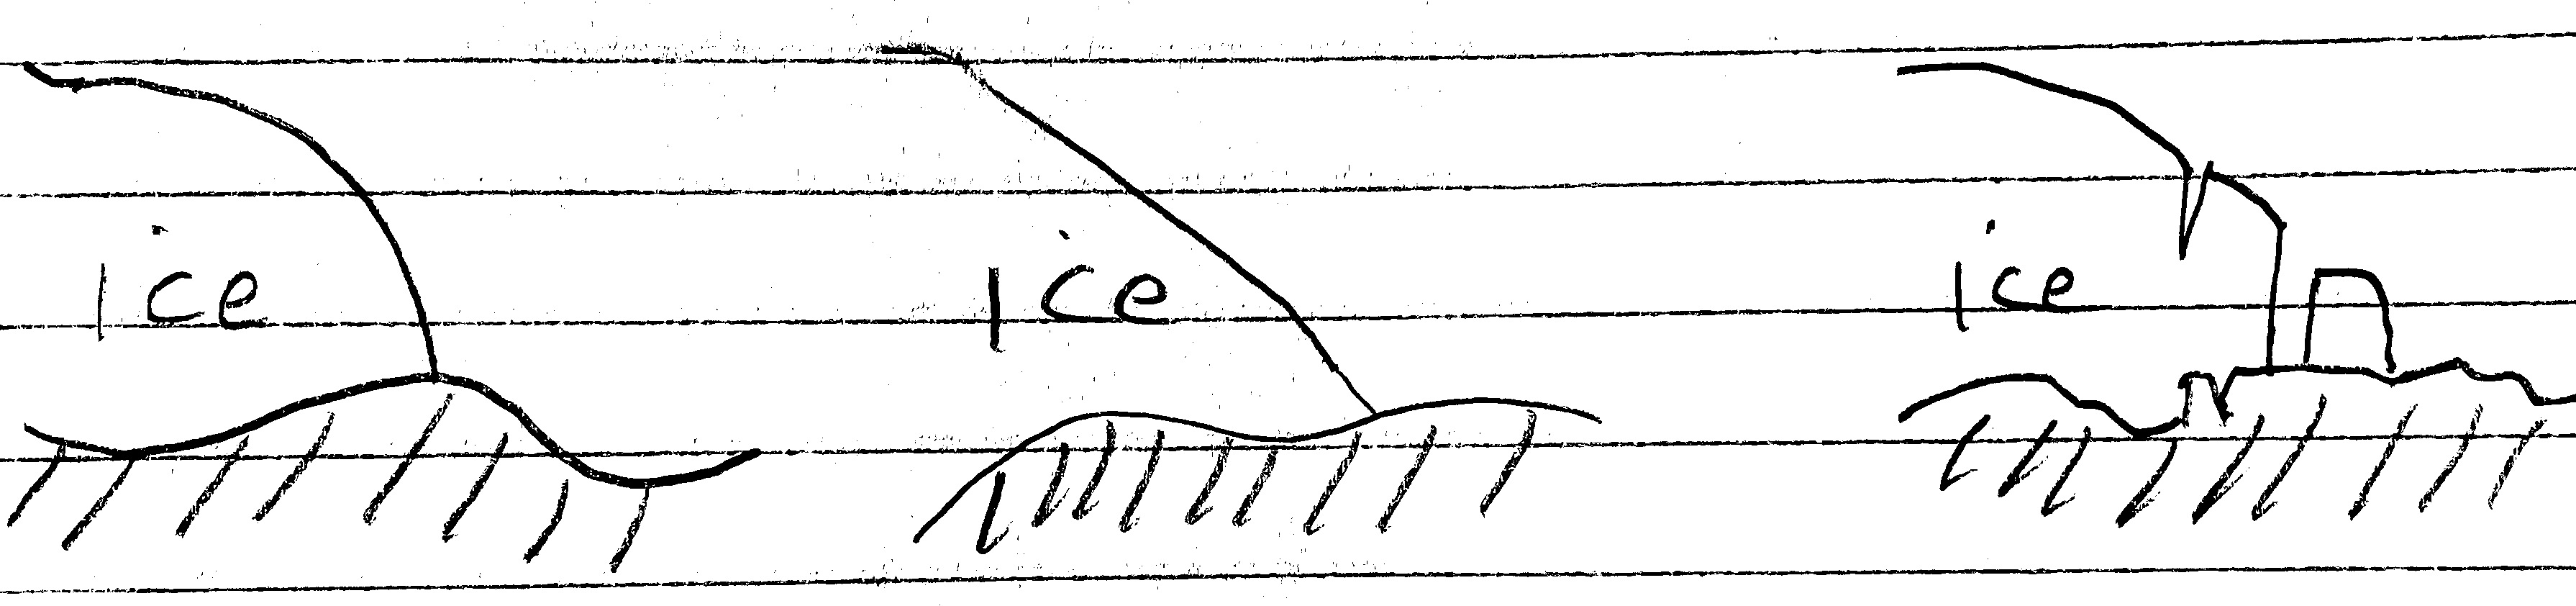
\includegraphics[width=0.8\textwidth]{figs/margins.jpg}
\end{center}
\caption{In which Sobolev space should we seek the surface elevation function?  This question relates to the theoretically-expected shape of the ice margin.  The shallow ice theory yields a fractional power shape (left).  Other glacier models hypothesize a ``wedge'' shape (center).  On the other hand, actual glacier margins often have overhangs, crevasses, and cliffs (right).}
\label{fig:margins}
\end{figure}

However, because margins are small features compared to the overall scale of glaciers and ice sheets, almost all modeling literature ignores overhangs and assumes instead that surface and bed elevation functions are well-defined; see \cite{IsaacStadlerGhattas2015,Jouvetetal2008,LofgrenAhlkronaHelanow2022,WirbelJarosch2020} among many examples.  Extending Stokes-based viscous models by allowing overhangs, and supplementing the momentum conservation model with an additional advected damage variable \cite{PralongFunk2005}, so that ice-cliff calving can occur via a stress-failure criterion, might provide a mechanism to explain how (nearly) well-defined surface elevation and thickness functions arise as solutions to the kind of models considered in this paper.

\subsection{Conjectural well-posedness for the continuum problem} \label{subsec:conjecture} Subsections \ref{subsec:explicit}--\ref{subsec:margin} have deployed imperfect arguments to explain why VI problem \eqref{eq:be:vi} could be well-posed.  With the understanding that this problem is non-trivial, for reasons sketched already, we now propose a mathematically-precise conjectural framework for well-posedness.  It uses a conjecture that the operator assigns sufficiently different results to inputs which are different in norm.

\begin{conjecture} \label{conj:b}
There exists $\rr>2$ so that Conjecture \ref{conj:a} holds and, with $\cX = W^{1,\rr}(\Omega)$ and $\cK=\{r\in\cX\,:\,r\ge b\}$ as before, furthermore it is true that, for each sufficiently-small step size $\Delta t>0$, there is a constant $\alpha>0$ and a power $\qq>1$ so that the operator in \eqref{eq:be:vi} satisfies
\begin{equation}
\ip{F_{\Delta t}(r) - F_{\Delta t}(s)}{r-s} \ge \alpha \|r-s\|_{\cX}^\qq \qquad \text{for all } r,s\in\cK. \label{eq:conj:b}
\end{equation}
\end{conjecture}

Inequality \eqref{eq:conj:b} is called $\qq$-\emph{coercivity}.  In the abstract VI context considered in Section \ref{sec:abstractestimate}, the fact that $F_{\Delta t}$ is both Lipschitz continuous (Lemma \ref{lem:philipschitz}) and $\qq$-coercive, over a closed and convex subset $\cK$ of a Banach space $\cX$, shows that the VI problem \eqref{eq:be:vi} is well-posed.  Thus Conjectures \ref{conj:a} and \ref{conj:b} are mathematically sufficient for well-posedness of each implicit time step problem.  We state this as a theorem.

\begin{theorem} \label{thm:stepwellposed}
Assume Conjectures \ref{conj:a} and \ref{conj:b} hold for $\rr>2$ and $\Delta t>0$.  Fix a bed elevation $b \in \cX=W^{1,\rr}(\Omega)$, which defines $\cK=\{r\in \cX\,:\,r\ge b\}$.  Suppose that the SMB function $a(t,x)$ is in $C([0,T]; L^{\rr'}(\Omega))$.  Suppose $s^{n-1}\in\cK$.  Then there exists a unique surface elevation $s\in\cK$ satisfying VI \eqref{eq:be:vi}.
\end{theorem}

\begin{proof}
Since $F_{\Delta t}$ is $\qq$-coercive it is also coercive and strictly-monotone (Section \ref{sec:abstractestimate}).  Let $q\in\cX$.  From definition \eqref{eq:be:source}, the given hypothesis on $a$, and H\"older's inequality,
\begin{equation}
|\ip{\ell^n}{q}| \le \left(\|s^{n-1}\|_{L^{\rr'}} + \Delta t \max_{t\in[t_{n-1},t_n]} \|a(t,\cdot)\|_{L^{\rr'}}\right) \|q\|_{L^\rr}.
\label{eq:sourcetermbound}
\end{equation}
Because $\|s^{n-1}\|_{L^{\rr'}}$ is finite by Sobolev's inequality, and because $\|q\|_{L^\rr} \le \|q\|_{\cX}$, it follows that the source term $\ell^n$ is in the dual space $\cX'$.  Now Corollary III.1.8 of \cite{KinderlehrerStampacchia1980} shows existence, and strict monotonicity shows uniqueness.
\end{proof}

Theorem \ref{thm:stepwellposed} addresses the well-posedness of a single implicit time-step problem over $[t_{n-1},t_n]$.  It is not sufficient to show well-posedness of the time-dependent problem over $[0,T]$.  The parabolic VI problem corresponding to the time-dependent NCP \eqref{eq:ncp} might also be well-posed, and this would be the minimum to analyze whether the implicit steps described here converge in the $\Delta t\to 0$ limit.

While practitioners of numerical ice sheet and glacier modeling using Stokes dynamics must expect conjectures like the above to hold, they may be difficult to prove despite the results in Sections \ref{sec:stokes} and \ref{sec:model}.  That greater progress has been made in the SIA case \cite{Calvoetal2003,JouvetBueler2012,PiersantiTemam2023} might be of assistance.  However, the geometry error bounds and results in the next two Sections only require Conjectures \ref{conj:a} and \ref{conj:b}.


\section{Abstract error estimate for a finite element approximation} \label{sec:abstractestimate}

We now consider the FE approximation of an abstract variational inequality (VI) problem.  We will return to glaciological VI problem \eqref{eq:be:vi} in Section \ref{sec:application}.

Let $\cV$ be a real reflexive Banach space with norm $\|\cdot\|$ and topological dual space $\cV'$.  Denote the dual pairing of $\phi \in \cV'$ and $v\in\cV$ by $\ip{\phi}{v} = \phi(v)$, and define the (Banach space) norm on $\cV'$ by $\|\phi\|_{\cV'} = \sup_{\|v\|=1} |\!\ip{\phi}{v}\!|$.  Let $\cK \subset \cV$ be a nonempty, closed, and convex subset, the constraint set; elements are said to be admissible.  For a continuous, but generally nonlinear, operator $f:\cK \to \cV'$, and a linear source $\ell\in \cV'$, the VI problem is to find $u\in \cK$ such that
\begin{equation}
\ip{f(u)}{v-u} \ge \ip{\ell}{v-u} \quad \text{for all } v\in \cK. \label{eq:vi}
\end{equation}
The best known example of such a problem is the obstacle problem for the Laplacian operator; see \cite{Ciarlet2002,Evans2010,KinderlehrerStampacchia1980} for its theory and FE analysis.

The following definitions are standard \cite[Chapter III]{KinderlehrerStampacchia1980}.  The definition of $\pp$-coercive has already appeared in Conjecture \ref{conj:b} (and in \cite{Bueler2021conservation}).

\begin{definition} \label{def:monotonepcoercive}
An operator $f:\cK \to \cV'$ is said to be \emph{monotone} if
\begin{equation}
\ip{f(v)-f(w)}{v-w} \ge 0 \qquad \text{for all } v,w \in \cK \label{eq:monotone}
\end{equation}
and \emph{strictly monotone} if equality in \eqref{eq:monotone} implies $v=w$.  It is \emph{coercive} if there is $w\in \cK$ so that for $v \in \cK$,
\begin{equation}
\frac{\ip{f(v)-f(w)}{v-w}}{\|v-w\|} \to +\infty \qquad \text{as } \|v\| \to +\infty. \label{eq:coercive}
\end{equation}
Let $\pp>1$.  The operator is \emph{$\pp$-coercive \cite{Bueler2021conservation}} if there exists $\alpha>0$ such that
\begin{equation}
\ip{f(v)-f(w)}{v-w} \ge \alpha \|v-w\|^\pp \qquad \text{for all } v,w \in \cK. \label{eq:pcoercive}
\end{equation}
\end{definition}

It is well-known that if $f:\cK \to \cV'$ is monotone and coercive, and also continuous on finite-dimensional subspaces, then VI \eqref{eq:vi} has a solution \cite[Corollary III.1.8]{KinderlehrerStampacchia1980}.  If $f$ is strictly monotone then the solution is unique.  If $f$ is $\pp$-coercive then it coercive and strictly monotone, so $\pp$-coercivity and continuity yield well-posedness for \eqref{eq:vi}.
% \cite{Peral1997} uniform continuity over bounded sets for p-Laplacian: Thm A.0.6

The following definition appeared in Conjecture \ref{conj:a}.

\begin{definition} \label{def:lipshitz}
For $\rho>0$ let $B_\rho = \{v\in \cV\,:\,\|v\|\le \rho\}$.  We say $f:\cK \to \cV'$ is \emph{Lipshitz on bounded subsets of $\cK$} if for every $\rho>0$ there is $C(\rho)>0$ so that if $v,w \in B_\rho \cap \cK$ and $z\in\cV$ then $|\ip{f(v)-f(w)}{z}| \le C(\rho) \|v-w\| \|z\|$, equivalently
\begin{equation}
\|f(v)-f(w)\|_{\cV'} \le C(\rho) \|v-w\| \quad \text{ for all } v,w \in B_\rho \cap \cK.  \label{eq:liponbounded}
\end{equation}
\end{definition}

Clearly, if $f$ is Lipshitz on bounded subsets then $f$ is continuous.  Note that definitions \ref{def:monotonepcoercive} and \ref{def:lipshitz} do not require $f$ to be defined on all of the vector space $\cV$, but only on $\cK$.

A key concept in the following theorem is that $f(u)-\ell$ is generally nonzero when $u$ solves \eqref{eq:vi}.  Instead, an NCP like \eqref{eq:ncp} or \eqref{eq:be:ncp} holds, at least in sufficiently regular cases.  (See \cite[Exercise 5.1.1]{Ciarlet2002} or \cite[section 7]{BuelerFarrell2024}, for example.)  Only for $u$ in the interior of $\cK$ should we expect equality (i.e.~$f(u)=\ell$).

An FE method for \eqref{eq:vi} solves a similar but finite-dimensional VI problem.  Suppose $\cV_h \subset \cV$ is a finite-dimensional subspace; typically $\cV_h$ consists of piecewise-polynomial and continuous functions defined on a mesh.  Define the FE constraint set $\cK_h\subset \cV_h$.  In general $\cK_h \nsubseteq \cK$.  Let $f_h:\cK_h\to\cV'$.  Generally $f_h\ne f$, because of quadrature and other approximations.  (The general case is considered below.)  The FE VI problem is
\begin{equation}
\ip{f_h(u_h)}{v_h-u_h} \ge \ip{\ell}{v_h-u_h} \quad \text{for all } v_h\in \cK_h. \label{eq:fe:vi}
\end{equation}
We assume that $f_h$ is $\pp$-coercive and continuous, and thus that this problem is also well-posed.

The following abstract error estimate extends \cite{Falk1974} and Theorem 5.1.1 in \cite{Ciarlet2002}.  Here we do not assume that $f$ is linear, nor that $\cK_h \subset \cK$ or $f_h=f$, and $f_h$ needs only be defined on $\cK_h$.  However, we must extend the domain of $f$ in \eqref{eq:vi} to include the finite element solution.

\begin{theorem} \label{thm:abstractestimate}  Suppose $u\in\cK$ solves \eqref{eq:vi} and $u_h\in\cK_h$ solves \eqref{eq:fe:vi}.  Define
\begin{equation}
\hcK = \overline{\Hull{(\cK \cup \cK_h)}}  \label{eq:convexhull}
\end{equation}
as the closure in $\cV$ of the convex hull of $\cK \cup \cK_h$, and suppose that $f$ can be extended to $\hcK$.  For $1<\pp<\infty$ assume $f$ is $\pp$-coercive over $\hcK$ with constant $\alpha>0$, and that it is Lipshitz on bounded sets of $\hcK$.  Let $R_h=\max\{\|u\|,\|u_h\|\}$.  Then there is a constant $c=c(\alpha,R_h)>0$ so that
\begin{align}
\|u-u_h\|^p &\le \quad \frac{2}{\alpha} \inf_{v\in\cK} \ip{f(u)-\ell}{v-u_h} \label{eq:abstractestimate} \\
   &\quad + \frac{2}{\alpha} \inf_{v_h\in\cK_h} \ip{f(u)-\ell}{v_h-u} \notag \\
   &\quad + \frac{2}{\alpha} \ip{f(u_h)-f_h(u_h)}{u_h} \notag \\
   &\quad + \inf_{v_h\in\cK_h} c \|v_h - u\|^\qq \notag
\end{align}
\end{theorem}

\begin{proof}  Consider arbitrary elements $v\in\cK$ and $v_h\in\cK_h$.  Rewrite VIs \eqref{eq:vi} and \eqref{eq:fe:vi}, as follows:
\begin{align*}
\ip{f(u)}{u}     &\le \ip{f(u)}{v} + \ell(u-v),  \\
\ip{f_h(u_h)}{u_h} &\le \ip{f_h(u_h)}{v_h} + \ell(u_h-v_h).
\end{align*}
It follows from $\pp$-coercivity over $\hcK$ and these inequalities that
\begin{align*}
\alpha \|u-u_h\|^\pp &\le \ip{f(u)-f(u_h)}{u-u_h} \\
  &= \ip{f(u)}{u} + \ip{f(u_h)}{u_h} - \ip{f(u)}{u_h} - \ip{f(u_h)}{u} \\
  &= \ip{f(u)}{u} + \ip{f_h(u_h)}{u_h} \\
  &\qquad - \ip{f(u)}{u_h} - \ip{f(u_h)}{u} + \ip{f(u_h)-f_h(u_h)}{u_h} \\
  &\le \ip{f(u)}{v} + \ell(u-v) + \ip{f(u_h)}{v_h} + \ell(u_h-v_h) \\
  &\qquad - \ip{f(u)}{u_h} - \ip{f(u_h)}{u} + \ip{f(u_h)-f_h(u_h)}{u_h} \\
  &= \ip{f(u)}{v-u_h} - \ell(v-u_h) + \ip{f(u_h)}{v_h-u} - \ell(v_h-u) \\
  &\qquad + \ip{f(u_h)-f_h(u_h)}{u_h} \\
  &= \ip{f(u)-\ell}{v-u_h} + \ip{f(u)-\ell}{v_h-u} \\
  &\qquad + \ip{f(u)-f(u_h)}{u-v_h} + \ip{f(u_h)-f_h(u_h)}{u_h}
\end{align*}
Since $u,u_h\in B_{R_h}$, by the Lipshitz assumption over $\hcK$ there is $C(R_h)>0$ so that
    $$\ip{f(u)-f(u_h)}{u-v_h} \le C(R_h) \|u-u_h\|\|u-v_h\|.$$
Noting $1<\pp,\qq<\infty$, now use Young's inequality with $\eps>0$ \cite[Appendix B.2]{Evans2010}:
\begin{align*}
\alpha \|u-u_h\|^\pp &\le \ip{f(u)-\ell}{v-u_h} + \ip{f(u)-\ell}{v_h-u} \\
  &\qquad + C(R_h) \left(\eps\|u-u_h\|^\pp + \tilde C(\eps) \|u-v_h\|^\qq\right) + \ip{f(u_h)-f_h(u_h)}{u_h}
\end{align*}
(Here $\tilde C(\eps) = (\eps \pp)^{-\qq/\pp} \qq^{-1}$.)  Choose $\eps>0$ so that $C(R_h) \eps \le \alpha/2$, and subtract:
\begin{align*}
\frac{\alpha}{2} \|u-u_h\|^\pp &\le \ip{f(u)-\ell}{v-u_h} + \ip{f(u)-\ell}{v_h-u} \\
  &\qquad + C(R_h) \tilde C(\eps) \|u-v_h\|^\qq + \ip{f(u_h)-f_h(u_h)}{u_h}
\end{align*}
Take infimums to show \eqref{eq:abstractestimate}.
\end{proof}

Consider $f(u)-\ell\in \cV'$ in Theorem \ref{thm:abstractestimate}.  In practical applications it might be a signed measure or a real-valued measurable function.  In such cases, the first two terms in estimate \eqref{eq:abstractestimate} include information about the sign of $f(u)-\ell$.  By contrast, the original Hilbert space result (\cite{Falk1974} and \cite[section 5.1]{Ciarlet2002}) compute norms and lose this information.  The following corollary to Theorem \ref{thm:abstractestimate} illustrates that norm-based approach.  We suppose that $\cV$ continuously and densely embeds in a larger Banach space $\cB$:
\begin{equation}
\cV \hookrightarrow \cB, \quad \overline{\cV} = \cB \label{eq:VembedsinB}
\end{equation}
Observe that $\cB' \subset \cV'$.  A standard example is where $\cV=W^{1,\qq}(\Omega)$ and $\cB=L^\qq(\Omega)$.  The proof of the following is immediate.

\begin{corollary}  \label{cor:abstractestimate:Bnorm}  In addition to the assumptions of Theorem \ref{thm:abstractestimate}, suppose that \eqref{eq:VembedsinB} holds, that $f(u_h)=f_h(u_h)$, and that $\|f(u)-\ell\|_{\cB'} < \infty$.  Then
\begin{align}
\|u-u_h\|^\pp &\le \frac{2}{\alpha} \|f(u)-\ell\|_{\cB'} \left( \inf_{v\in\cK} \|v-u_h\|_{\cB} +   \inf_{v_h\in\cK_h} \|v_h-u\|_{\cB} \right) \label{eq:abstractestimate:Bnorm} \\
   &\qquad + \inf_{v_h\in\cK_h} c \|v_h - u\|^\qq \notag
\end{align}
\end{corollary}

The convex hull operation \eqref{eq:convexhull} is not needed if the nonlinear operator $f$ is defined on all of $\cV$ and if $f_h=f$.  That is, \eqref{eq:abstractestimate} holds if one replaces $\hcK$ with $\cV$ itself for the domain of $f$.  Furthermore, for \emph{linear} operators defined in this way, Theorem \ref{thm:abstractestimate} reduces to the FE error estimate for VIs by Falk \cite{Falk1974}.  Specifically, suppose $\ip{f(v)}{w}=a(v,w)$ is actually bilinear, $\cV$-elliptic, and continuous on a Hilbert space $\cV$.  Define $A:\cV\to\cV'$, a bounded linear operator, by $Av(w) = a(v,w)$.  Observe that continuity for $a(v,w)$ implies Lipshitz on bounded sets \eqref{eq:liponbounded} for $A$.  Suppose that $\cV\hookrightarrow \cH$ and $\overline{\cV} = \cH$ for some larger Hilbert space $\cH$, and that $\|Au-\ell\|_{\cH'} < \infty$ so that, up to isomorphism, $Au-\ell \in \cH$.  Then Corollary \ref{cor:abstractestimate:Bnorm} reduces to Theorem 1 in \cite{Falk1974} and Theorem 5.1.1 in \cite{Ciarlet2002}.

As observed in \cite{Ciarlet2002}, the quantity in estimates \eqref{eq:abstractestimate} and \eqref{eq:abstractestimate:Bnorm} which involves $v-u_h$, for $v\in\cK$, is generally nonzero in obstacle problems where $\cK_h \nsubseteq \cK$.  (This is relevant to glacier models tracking the surface elevation, as opposed to thickness.)  In fact, suppose that $\cK=\{v \in \cV\,:\,v\ge \psi\}$, $\psi_h$ is an interpolant of $\psi$, and $\cK_h=\{v_h \in \cV_h\,:\,v_h\ge \psi_h\}$.  Observe that, while $\psi_h(x_j)=\psi(x_j)$ for interpolation nodes $x_j$, generally $\psi_h(x) \ge \psi(x)$ does not hold for all $x\in\Omega$, even if $\psi$ is arbitrarily smooth.  In other words, nodal admissiblity does not imply admissibility (Figure \ref{fig:nonadmissible}).

\begin{figure}
\begin{center}
FIXME figure like Ciarlet Figure 5.1.3 %\includegraphics[width=0.8\textwidth]{figs/xxx.jpg}
\end{center}
\caption{Nodal admissibility generally does not imply admissibility.  Thus, if $\phi_h$ is the FE interpolant of an obstacle $\psi$, it is possible that $\cK_h \nsubseteq \cK$.}
\label{fig:nonadmissible}
\end{figure}

The following corollary is relevant to glacier models solving for ice thickness, as opposed to surface elevation.  In such cases $\cK = \{v\ge 0\}$ consists of all nonnegative functions and $\cK_h=\cK\cap\cV_h$.

\begin{corollary}  \label{cor:abstractestimate:subset}  Keeping the assumptions of Theorem \ref{thm:abstractestimate}, suppose also that $\cK_h \subset \cK$, and that $f(u_h)=f_h(u_h)$.  Then
\begin{equation}
\|u-u_h\|^\pp \le  \inf_{v_h\in\cK_h} \left\{\frac{2}{\alpha} \ip{f(u)-\ell}{v_h-u} + c \|v_h - u\|^\qq\right\}. \label{eq:abstractestimate:subset}
\end{equation}
If also the assumptions of Corollary \ref{cor:abstractestimate:Bnorm} hold then
\begin{equation}
\|u-u_h\|^\pp \le \inf_{v_h\in\cK_h} \left\{\frac{2}{\alpha} \|f(u)-\ell\|_{\cB'} \|v_h-u\|_{\cB} + c \|v_h-u\|^\qq\right\} \label{eq:abstractestimate:subset:Bnorm}
\end{equation}
Finally, if additionally $f(u)=\ell$, for example if $u$ is in the interior of $\cK$, then
\begin{equation}
\|u-u_h\| \le \tilde c \inf_{v_h\in\cK_h} \|v_h-u\|^{\qq/\pp} \label{eq:abstractestimate:subset:Cea}
\end{equation}
\end{corollary}

Note that \eqref{eq:abstractestimate:subset:Cea} is Cea's lemma \cite[Theorem 2.4.1]{Ciarlet2002} translated to Banach spaces.  Also, in \eqref{eq:abstractestimate:subset:Cea} we have reduced to the PDE case where there is no active set or free boundary.  In the glacier context, \eqref{eq:abstractestimate:subset:Cea} corresponds to the case where the entire domain $\Omega$ is covered in ice.


\section{Application of the estimate} \label{sec:application}

FIXME apply Theorem \ref{thm:abstractestimate} and talk through what happens

FIXME accomodate the barrier theory from \cite{Bueler2021conservation}


\section{Demonstration of computable geometry error bounds} \label{sec:demo}

FIXME use stuff from multilevel-stokes-geometry


\section{Conclusion} \label{sec:conclusion}

FIXME


\bibliographystyle{siamplain}
\bibliography{estimate}

\end{document}
